\documentclass[11pt,letterpaper,onecolumn]{article}

\usepackage[utf8]{inputenc}
\usepackage[spanish]{babel}
\usepackage{float}
\usepackage{xcolor}
\usepackage{verbatim}
\usepackage{mwe}
\usepackage{charter}
\usepackage{afterpage}
\usepackage{amsmath}
\usepackage{appendix}
\usepackage{ragged2e}
\usepackage{array}
\usepackage{etoolbox}
\usepackage{fancyhdr}
\usepackage{booktabs}
\usepackage{arydshln}
\usepackage[justification=justified,singlelinecheck=false,labelfont=bf,format=plain]{caption}
\usepackage[justification=justified,singlelinecheck=false,labelfont=bf,format=plain]{subcaption}
\usepackage{enumitem}
\usepackage[bottom=2.5cm,top=2.0cm,left=2.0cm,right=2.0cm]{geometry}
\usepackage{graphicx}
\usepackage{indentfirst}
\usepackage{mathtools}
\usepackage{multirow}
\usepackage{pdfpages}

\usepackage{subfiles}
\usepackage[compact]{titlesec}
\usepackage{blindtext}
\usepackage{stfloats}
\usepackage{lipsum} 


\renewcommand{\familydefault}{\rmdefault}

\newcommand\blankpage{
    \null
    \thispagestyle{empty}
    \addtocounter{page}{0}
    \newpage}

\newcolumntype{L}[1]{>{\raggedright\let\newline\\arraybackslash\hspace{0pt}}m{#1}}
\newcolumntype{C}[1]{>{\centering\let\newline\\arraybackslash\hspace{0pt}}m{#1}}
\newcolumntype{R}[1]{>{\raggedleft\let\newline\\arraybackslash\hspace{0pt}}m{#1}}

    \setlist[itemize,1]{label=$\bullet$}
    \setlist[itemize,2]{label=$\circ$}
    \setlist[itemize,3]{label=$-$}
    \setlist{nosep}

\setlength{\columnsep}{30pt}

\titlelabel{\thetitle.\quad}

\pagestyle{fancy}
\fancyhf{}
      
\fancyfoot{}
\fancyfoot[C]{\thepage} % page
\renewcommand{\headrulewidth}{0mm} % headrule width
\renewcommand{\footrulewidth}{0mm} % footrule width

\makeatletter
\patchcmd{\headrule}{\hrule}{\color{black}\hrule}{}{} % headrule
\patchcmd{\footrule}{\hrule}{\color{black}\hrule}{}{} % footrule
\makeatother

\definecolor{blueM}{cmyk}{1.0,0.49,0.0,0.47}

%%%%%%%%%%%%%%%%%%%%%%%%%%%%%%%%%%%%%%%%%%%%%%%%%%%%%%%%%%%%%%%%%%%%%%%%%%%%%%%%%%%%%%%%%%%%%%%%%%%%%%%%%%%%%%%%%%%%%%%%%%%%%%%%%%%%%%%%%%%%%%%%%%%%%%%%%%%%%%%%%%%%%%%%%%%%%%%%%%%%%%%%%%%%%%%%%%%%%%%%%%%%%%
%%%%%%%%%%%%%%%%%%%%%%%%%%%%%%%%%%%%%%%%%%%%%%%%%%%%%%%%%%%%%%%%%%%%%%%%%%%%%%%%%%%%%%%%%%%%%%%%%%%%%%%
\chead[C]{
      \begin{tabular}{m{1.5cm}m{11.5cm}m{2.5cm}}
      
\includegraphics[height=1.5cm]{logo.png}
      &
      \centering
     \fcolorbox{white}{white}{\fbox{\begin{minipage}{11.5cm}
     \centering
     \textcolor{blueM}{ Prácticas Programación y Control}
     \end{minipage}}}
         &
        \centering
         \tiny{ \vspace{3.5mm} Grado en Física \\  %para usar en otras carreras consulte a su coordinador
%%%%%%%%%%%%%%%%%%%%%%%%%%%%%%%%%%%%%%%%%%%%%%%%%%%%%%%%%%%%%%%%%%%%%%%%%%%%%%%%%%%%%%%%%%%%%%%%%
             %elija el que corresponda ejemplo :  Modular : I
%%%%%%%%%%%%%%%%%%%%%%%%%%%%%%%%%%%%%%%%%%%%%%%%%%%%%%%%%%%%%%%%%%%%%%%%%%%%%%%%%%%%%%%%%%%%%%%%%
            Página \thepage \hspace{1pt} de 8
          }\tabularnewline
%          \hline
          \end{tabular}%
    }
    
\begin{document}


\hspace{25pt}
\begin{minipage}{0.75\textwidth}
\begin{center}
	
	\vspace{5mm}

	\Large{\textbf{Asignatura de Proyectos. 3º Física}} %
    \\ 
    \large{\textbf{Martín Romero, Álvaro}. \textcolor{blueM}{f82maroa@uco.es}} % Si solo hay un autor borrar el apartado sin borrar el ultimo }\\ 
   \\ 
    \vspace{2mm}
    \fontsize{0.35cm}{0.5cm}\selectfont \textit{Departamento de Física, UCO, Universidad de Córdoba}
    \vspace{1mm} 
    
    \today % FECHA

\end{center}
\end{minipage}

\small

\vspace{11pt}

\centerline{\rule{0.95\textwidth}{0.4pt}}

\begin{center}
    
    \begin{minipage}{0.9\textwidth}
        % RESUMEN
	    \noindent \textbf{Resumen:} En esta  práctica conoceremos como usar el programa \textbf{Microsoft Project} para gestionar un proyecto  para la adquisición de un software de gestión  de embarque de un aeropuerto 
    
        \vspace{4mm}
        % PALABRAS CLAVE
    
    \end{minipage}
    
\end{center}
\centerline{\rule{0.95\textwidth}{0.4pt}}
\vspace{15pt}
Lo primero que debemos hacer es abrir el programa \textbf{Microsoft Project}. Una vez abierto, metemos los datos de las actividades que son necesarias para realizar el proyecto. Esto es, escribimos la letra asignada a cada actividad, la descripción de cada actividad y el tiempo estimado. \\
\\
En \textit{Proyecto/Información del Proyecto/ Tiempo de inicio} podemos configurar el tiempo de inicio para nuestro proyecto, en nuestro caso, el \textbf{13 de marzo de 2019}. Una vez rellenado todas las casillas vemos las siguientes columnas (La columna actividad crítica la obviamos por ahora, haciendo de su uso posteriormente):
\begin{figure}[H]
\begin{center}
    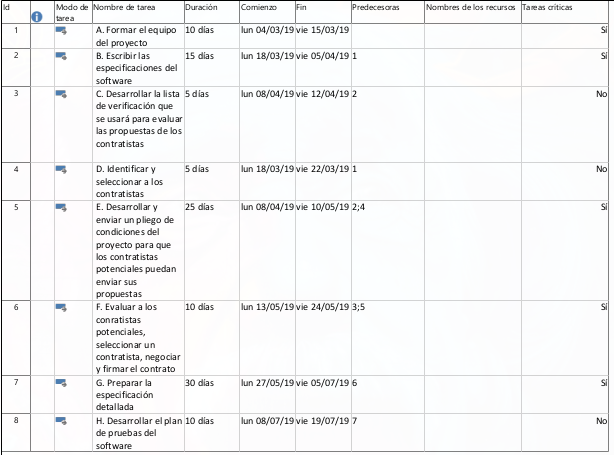
\includegraphics[scale=0.9]{actividad1.png}
\end{center}
\label{fig:}
\end{figure}
\begin{figure}[H]
\begin{center}
    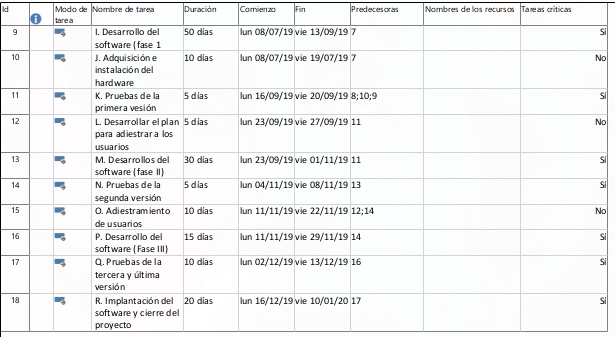
\includegraphics[scale=0.9]{actividad2.png}
\end{center}
\label{fig:}
\end{figure}


Para la información que nos piden, vemos necesario realizar un informe con todos esos datos. Para ello, desde \textbf{Microsoft Project} realizamos un \textit{informe} y pulsando en el informe general podemos ir añadiendo variables y cambiar el nombre de algunas que nos dan la información que queremos pero nos la introduce con otro nombre. El informe completo queda tal que:

\begin{figure}[H]
\begin{center}
    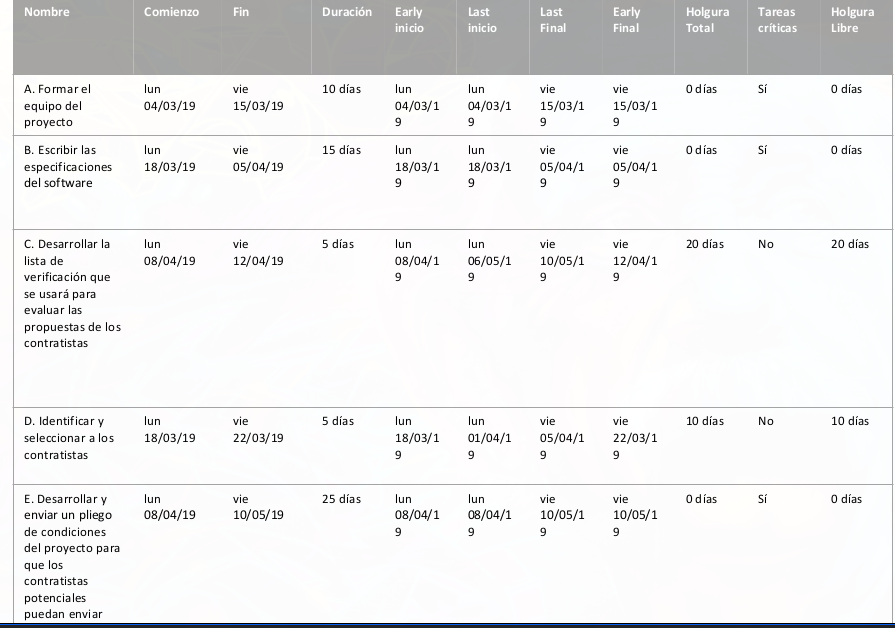
\includegraphics[scale=0.6]{informe1.png}
\end{center}
\label{fig:}
\end{figure}
\begin{figure}[H]
\begin{center}
    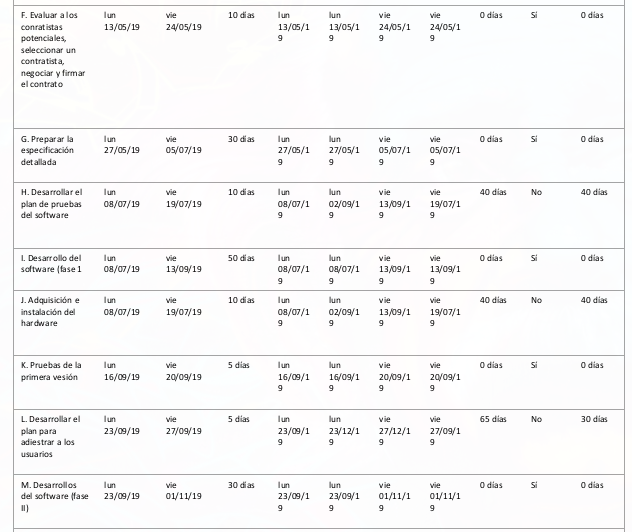
\includegraphics[scale=1]{informe2.png}
\end{center}
\label{fig:}
\end{figure}
\begin{figure}[H]
\begin{center}
    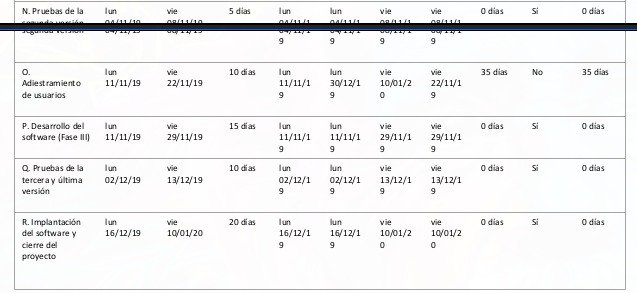
\includegraphics[scale=1]{informe3.png}
\end{center}
\label{fig:}
\end{figure}

A continuación vamos a comentar los resultados hallados gracias al informe hecho por el programa incluyendo los datos de nuestro proyecto:
\\

\begin{itemize}
    \item{\textbf{Tiempo más temprano de inicio:}} Esto queda indicado en el informe con '\textit{Early inicio}' y es el día de inicio de cada actividad más optimista, es decir, suponiendo que todas las tareas anteriores acaben el día señalado. \\
\\


    \item{\textbf{Tiempo más tardío de inicio:}} Esto en el informe es dado por '\textit{Tiempo Last final}'.Este es el tiempo más pesimista para que comience una tarea. Para las actividades que corresponden al camino crítico, el tiempo early y last de inicio coinciden, habiendo por consiguiente un retraso en el proyecto final si estas actividades retrasan sus fechas de inicio.\\
\\
Un ejemplo de tiempo early de inicio es el día 8/04 para la actividad C, la duración last de inicio es el día 6/05 para la actividad. Como vemos, la actividad C se puede desarrollar en un margen de tiempo, esto indica que no pertenece al camino crítico.
\\

    \item{\textbf{Tiempo más temprano final:}} Esto es '\textbf{Early Final}', es la fecha más optimista a la cual la tarea es acabada. Si la tarea se retrasa más de la fecha early final, esto no tiene porqué suponer un retraso en el proyecto\\
\\
    \item{\textbf{Tiempo más tardío final:}} Esto es '\textbf{Last Final}', es la fecha más pesimista a la cual acaba la tarea. Esto es, el límite para que la actividad no retrase el proyecto, debe acabarse antes de esta fecha last final. \\
\\
Un ejemplo de tiempo early final es el día 10/05 para la actividad E. Para esta actividad, el tiempo last final es el día 10/05. Estos días coincide, es decir, la actividad debe terminarse si o si ese día si no queremos que el tiempo total del proyecto se retrase, esta actividad corresponde a una actividad del camino crítico.
\\
\item{\textbf{Camino Crítico:}} El camino crítico es el camino recorrido por las tareas para que el proyecto pueda acabar lo antes posible. Si una actividad del camino crítico se retrasa, perjudica a todo el proyecto aumentando la duración de este el tiempo que se retrase tal tarea. Por ello, las holguras de las actividades que pertenecen al camino crítico son nulas. El camino crítico para este proyecto es:
    \[
    A-B-E-F-G-I-K-M
    .\] 
A continuación vamos a realizar una tabla en Excel para calcular las holguras de diferentes tipos junto a cada actividad, así vemos que el camino crítico concuerda con lo que nos da el programa:
\begin{table}[htbp]
    \centering
    \begin{tabular}{|c|ccccccccc|}
        \hline
        $Actividad$ & $d$ & $t_i$ & $t_j$ & $t_i*$ & $t_j*$ & $H_i$ & $H_j$ & $H^t_{ij}$ & $H_{ij}^t$ \\ \hline
        1-2 A & 10 & 0 & 10 & 0 & 10 & 0 & 0 & 0 & 0 \\ \hline
        2-3 B & 15 & 10 & 25 & 10 & 25 & 0 & 0 & 0 & 0 \\ \hline
        2-4 D & 5 & 10 & 25 & 10 & 25 & 0 & 0 & 10 & 10 \\ \hline
        3-4 F1 & 0 & 25 & 25 & 25 & 25 & 0 & 0 & 0 & 0 \\ \hline
        3-5 C & 5 & 25 & 50 & 25 & 50 & 0 & 0 & 20 & 20 \\ \hline
        4-5 E & 25 & 25 & 50 & 25 & 50 & 0 & 0 & 0 & 0 \\ \hline
        5-6 F & 10 & 50 & 60 & 50 & 60 & 0 & 0 & 0 & 0 \\ \hline
        6-7 G & 30 & 60 & 90 & 60 & 90 & 0 & 0 & 0 & 0 \\ \hline
        7-8 H & 10 & 90 & 100 & 90 & 140 & 0 & 40 & 40 & 0 \\ \hline
        7-9 J & 10 & 90 & 100 & 90 & 140 & 0 & 40 & 40 & 0 \\ \hline
        7-10 I & 50 & 90 & 140 & 90 & 140 & 0 & 0 & 0 & 0 \\ \hline
        8-10 F2 & 0 & 100 & 140 & 140 & 140 & 40 & 0 & 40 & 40 \\ \hline
        9-10 F3 & 0 & 100 & 140 & 140 & 140 & 40 & 0 & 40 & 40 \\ \hline
        10-11 K & 5 & 140 & 145 & 140 & 145 & 0 & 0 & 0 & 0 \\ \hline
        11-12 M & 30 & 145 & 175 & 145 & 175 & 0 & 0 & 0 & 0 \\ \hline
        11-14 L & 5 & 145 & 180 & 145 & 215 & 0 & 35 & 65 & 30 \\ \hline
        12-13 N & 5 & 175 & 180 & 175 & 180 & 0 & 0 & 0 & 0 \\ \hline
        13-14 F4 & 0 & 180 & 180 & 180 & 215 & 0 & 35 & 35 & 0 \\ \hline
        13-15 P & 15 & 180 & 195 & 180 & 195 & 0 & 0 & 0 & 0 \\ \hline
        14-17 O & 10 & 180 & 225 & 215 & 225 & 35 & 0 & 35 & 35 \\ \hline
        15-16 Q & 10 & 195 & 205 & 195 & 205 & 0 & 0 & 0 & 0 \\ \hline
        16-17 R & 20 & 205 & 225 & 205 & 225 & 0 & 0 & 0 & 0 \\ \hline
    \end{tabular}
    \label{}
    \captionsetup{justification=centering}
    \caption{Tener en cuenta que los tiempos están dados en días. Hemos acumulado los días para hacer más sencilla la cuenta total. }    
\end{table}

\item{\textbf{Holgura Total:}}La holgura total es el tiempo que se puede retrasar una tarea sin afectar a la duración del pryecto. Para el camino crítico la holgura total debe ser nula. \\
\\
\item{\textbf{Holgura Libre:}}La holgura libre es el tiempo que se puede retrasar una tarea sin que afecte a la fecha de comienzo de las tareas sucesoras. Igual que en todas las holguras, esta holgura para el camino crítico debe ser nula.\\
\\
Tener en cuenta que estas holguras no pueden ser negativas, la única holgura posible negativa es la independiente; ni la libre ni la total pueden serlo. \\
\\

\item{\textbf{Fecha finalización del proyecto:}} La fecha de finalización del proyecto viene dada por el último día de la actividad que acaba el camino crítico, esta fecha es el \textbf{16/12/2019}. \\
\\
\item{\textbf{Fecha de comienzo prevista para acabar el 22/11/2019.}} Para ello pinchamos en \textit{Proyecto/Información del Proyecto/ Tiempo final} y cambiamos la fecha de finalización del proyecto al 22/11/2019. La fecha que nos marca para inciar el proyecto con todas las actividades con su duración y siguiendo el camino crítico es el \textbf{14/01/2019}. Lo vemos en la siguiente imagen:
    \begin{figure}[H]
        \centering
        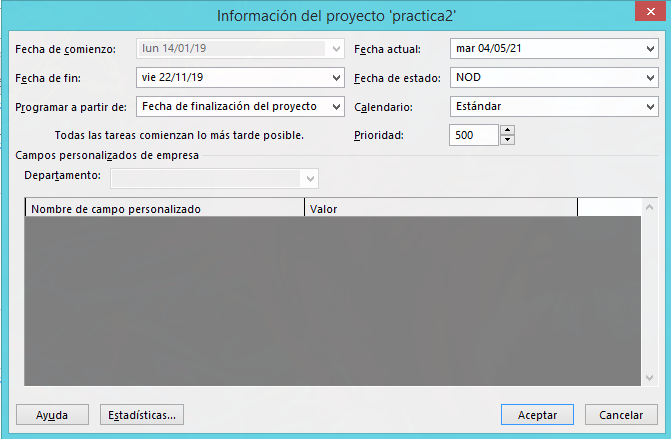
\includegraphics[width=0.8\textwidth]{g.png}
        \label{fig:g-png}
    \end{figure}

\item{\textbf{Informes interesantes:}}
    Un informe bastante interesante es el llamado informe de estado de la tarea, donde nos muestran de forma muy esquemática y fácil de ver los estados de la tarea junto con un unas flechas de prerelaciones donde podemos obtener mucha información del proyecto en una sola gráfica.\\
\\
Parte de este gráfico lo adjuntamos a continuación:
\begin{figure}[H]
    \centering
    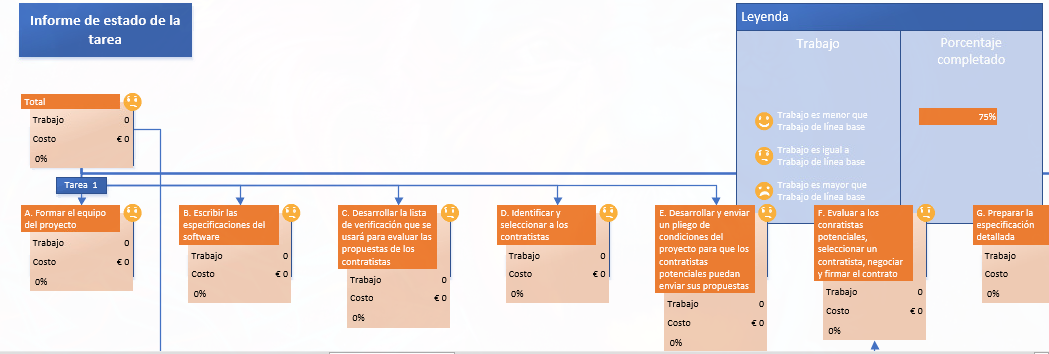
\includegraphics[width=0.8\textwidth]{informegrafico.png}
    \label{fig:}
\end{figure}
\end{itemize}
Además, el diseño gráfico no cansa para nada la vista y es agradable al ver. Sin duda el informe que más me ha llamado la atención y que usaría para futuros proyectos para poder ver todo de forma más clara y al alcance, que es el objetivo de un buen informe de un proyecto 

hola que tal
\end{document}

